\chapter{Fatiando a Terra}

\begin{quotation}
    \textit{%
    ``El cómputo en la ciencia ha evolucionado no solo porque el software lo ha
    hecho, sino porque nosotros, como científicos, estamos haciendo mucho más
    que solo aritmética de punto flotante.''
    }
\end{quotation}
\begin{flushright}
Fernando Pérez, \textit{PyCon Canada 2012}
\end{flushright}

\section{Introducción}

Desde su invención, las computadoras han sido puestas a disposición de la
comunidad científica con el objetivo de resolver problemas que resultaban
inalcanzables.
Esta interacción entre una tecnología de vanguardia y el ambiente científico
generaba no solo beneficios para esta última parte, sino también una gran
retroalimentación.
Se desarrollaron lenguajes de programación especialmente diseñados para
resolver problemas numéricos junto con interfaces que facilitaran la
visualización y manipulación de datos científicos.
La relación entre ciencia y las herramientas computacionales se desarrolló tan
rápido que fue necesario crear el término \emph{computación científica} para
diferenciarla de los otros usos que se estaban gestando para las computadoras
(telecomunicaciones, fines comerciales, sistemas estatales de datos, etc.).
Hoy en día es imposible imaginar una ciencia que no necesite de las
herramientas computacionales para su avance y la resolución de los problemas
que enfrenta en la actualidad.

A medida que los problemas científicos se vuelven cada vez más complejos de
resolver,
también lo hacen las tareas necesarias para hacerlo.
Mantenerse actualizado en los últimos conocimientos en la materia, adquirir
nuevos datos, desarrollar el software necesario para procesarlos y finalmente
generar un nuevo conocimiento se presenta como un desafío titánico para ser
desempeñado por una persona o por apenas un puñado de investigadores.
La complejidad actual de la ciencia requiere que el clásico flujo de trabajo
científico se distribuya a lo ancho de la comunidad, ofreciendo productos
o soluciones para cada una de sus etapas, que puedan ser utilizados libremente
por otros investigadores y otras investigadoras, que a su vez puedan
modificarlos y volver a distribuirlos en caso de desearlo.
En resumen, los problemas científicos actuales requieren soluciones
comunitarias y colaborativas, tanto para dar respuestas a las preguntas
fundamentales, así como para desarrollar herramientas que faciliten la
resolución de estos problemas.

Los movimientos de Software Libre y de código abierto que comenzaron
a proliferarse durante las décadas de los 80 y 90 tuvieron una fuerte raíz en
el ámbito científico.
Muchos científicos y científicas comenzaron a desarrollar herramientas
computacionales a partir de necesidades propias de sus investigaciones que
luego las distribuyeron bajo licencias de Software Libre y de código abierto.
Dentro de las ciencias de la Tierra podemos hallar Seismic Unix
\citep{seismicunix}, cuyo desarrollo comenzó a finales de la década del 70
y está disponible bajo una licencia BSD Clause-3; y GMT (Generic Mapping Tool)
\citep{gmt1991,gmt2019}, creado en 1988 por Paul Wessel y Walter H.F.
Smith y lanzado bajo la GNU Lesser General Public License%
\footnote{%
    \url{https://en.wikipedia.org/wiki/GNU_Lesser_General_Public_License}%
}
en 1991.

A inicios de la década del 2000 se comienzan a desarrollar herramientas
especialmente orientadas a aplicaciones científicas y de cálculo numérico que
hacían uso del lenguaje de programación Python, creado por Guido van Rossum una
década atrás.
En 2001 se lanza IPython \citep{perez2007}, un intérprete de comandos
interactivo, cuyo objetivo es facilitar la forma en la cual los usuarios y las
usuarias operan con sus datos.
En el mismo año ve la luz la primera versión de SciPy \citep{scipy2020}, una
librería con módulos de optimización, álgebra lineal, integración,
interpolación, resolución de ecuaciones diferenciales, aplicación de
Transformada de Fourier, entre otros.
En 2003 aparece la primera versión de Matplotlib \citep{matplotlib2007}, una
librería para realización de gráficos y visualización de datos con una \ac{API}
orientada a objetos.
En 2006, se bautiza a la librería NumPy \citep{numpy2020}, heredera de Numeric,
dando soporte a operaciones con arreglos al lenguaje Python, para lo cual no
había sido diseñado.

Estas herramientas comenzaron a ser utilizadas dentro de diferentes ambientes
científicos y los entornos que ofrecía Python comenzaron a perfilarse como un
excelente ecosistema para la computación científica
\citep{travis2007,millman2011,perez2011}.

La segunda década del nuevo milenio comenzó a vislumbrar una explosión en la
cantidad de aplicaciones y nuevos desarrollos de software alrededor de estas
nuevas herramientas.
Se destacan proyectos como Jupyter \citep{jupyter2016}, lanzado en 2016, que
logró introducir un nuevo tipo de forma de interactuar con código de
investigación: los \emph{Jupyter Notebooks}, que facilitan no solo la
experimentación, sino la comunicación de los procesos y resultados científicos
junto con la reproducibilidad de los mismos.
Librerías como Pandas \citep{pandas2010}, que ofrece herramientas para la
manipulación y análisis de datos; scikit-learn \citep{sklearn2011},
especialmente orientada a la aplicación de algoritmos de aprendizaje
automático; SymPy \citep{sympy2017} para cálculo simbólico; entre otras.
Surge también Anaconda\footnote{\url{https://www.anaconda.com}}, una
distribución de Python orientada específicamente a la ciencia de datos,
aprendizaje automático e investigaciones científicas; facilitando la
instalación del intérprete y las múltiples librerías en diferentes plataformas
y sistemas operativos.

En este capítulo expondremos las  características del proyecto
Fatiando a Terra, del cual el autor de esta Tesis forma parte del grupo de
desarrolladores.
Recorreremos su historia y cómo, dentro de su marco, se construyen herramientas
computacionales con aplicaciones directas en geofísica, particularmente sobre
temáticas relacionadas a métodos potenciales.
Enumeraremos las prácticas de desarrollo de software aprendidas y aplicadas en
la construcción del proyecto, y qué beneficio han traído a la generación de
investigaciones científicas reproducibles.
También exploraremos de qué manera existe una retroalimentación entre los
proyectos de software científico y las investigaciones que estos permiten.
Finalmente bosquejaremos un conjunto de ideas a implementar a futuro,
definiendo los nuevos caminos que el proyecto debe tomar en función del
ambiente científico actual.


\section{Historia}

Los orígenes del proyecto se remontan a finales de la década del 2000, cuando
Leonardo Uieda y Vanderlei Oliveira Jr. junto a otros estudiantes se
encontraban cursando los últimos años del Bachillerato en Geofísica
(\emph{Bacharelado em Geofísica}) en la Universidade de São Paulo.
En este contexto surge la idea de implementar una alternativa propia a los
software de modelado gravimétrico 2D comerciales.
Tras asistir a cursos dictados por
Software Carpentry\footnote{%
    \url{https://software-carpentry.org}
}
en Canadá, Leonardo Uieda adquiere mayores conocimientos en el uso de sistema
de control de versiones junto a otras mejores prácticas para el desarrollo de
Software y regresa con nuevas ideas para el proyecto.
De vuelta en São Paulo, se gesta un diagrama de un posible diseño para este
proyecto (fig.~\ref{fig:talwani-idea}).
La idea finalmente se desarrolla mediante una implementación del método de
\citet{talwani1959} para modelado directo de polígonos 2D, y la posterior
construcción de una interfaz gráfica escrita en C que más tarde se
reimplementaría en Python.

\begin{figure}[h]
    \centering
    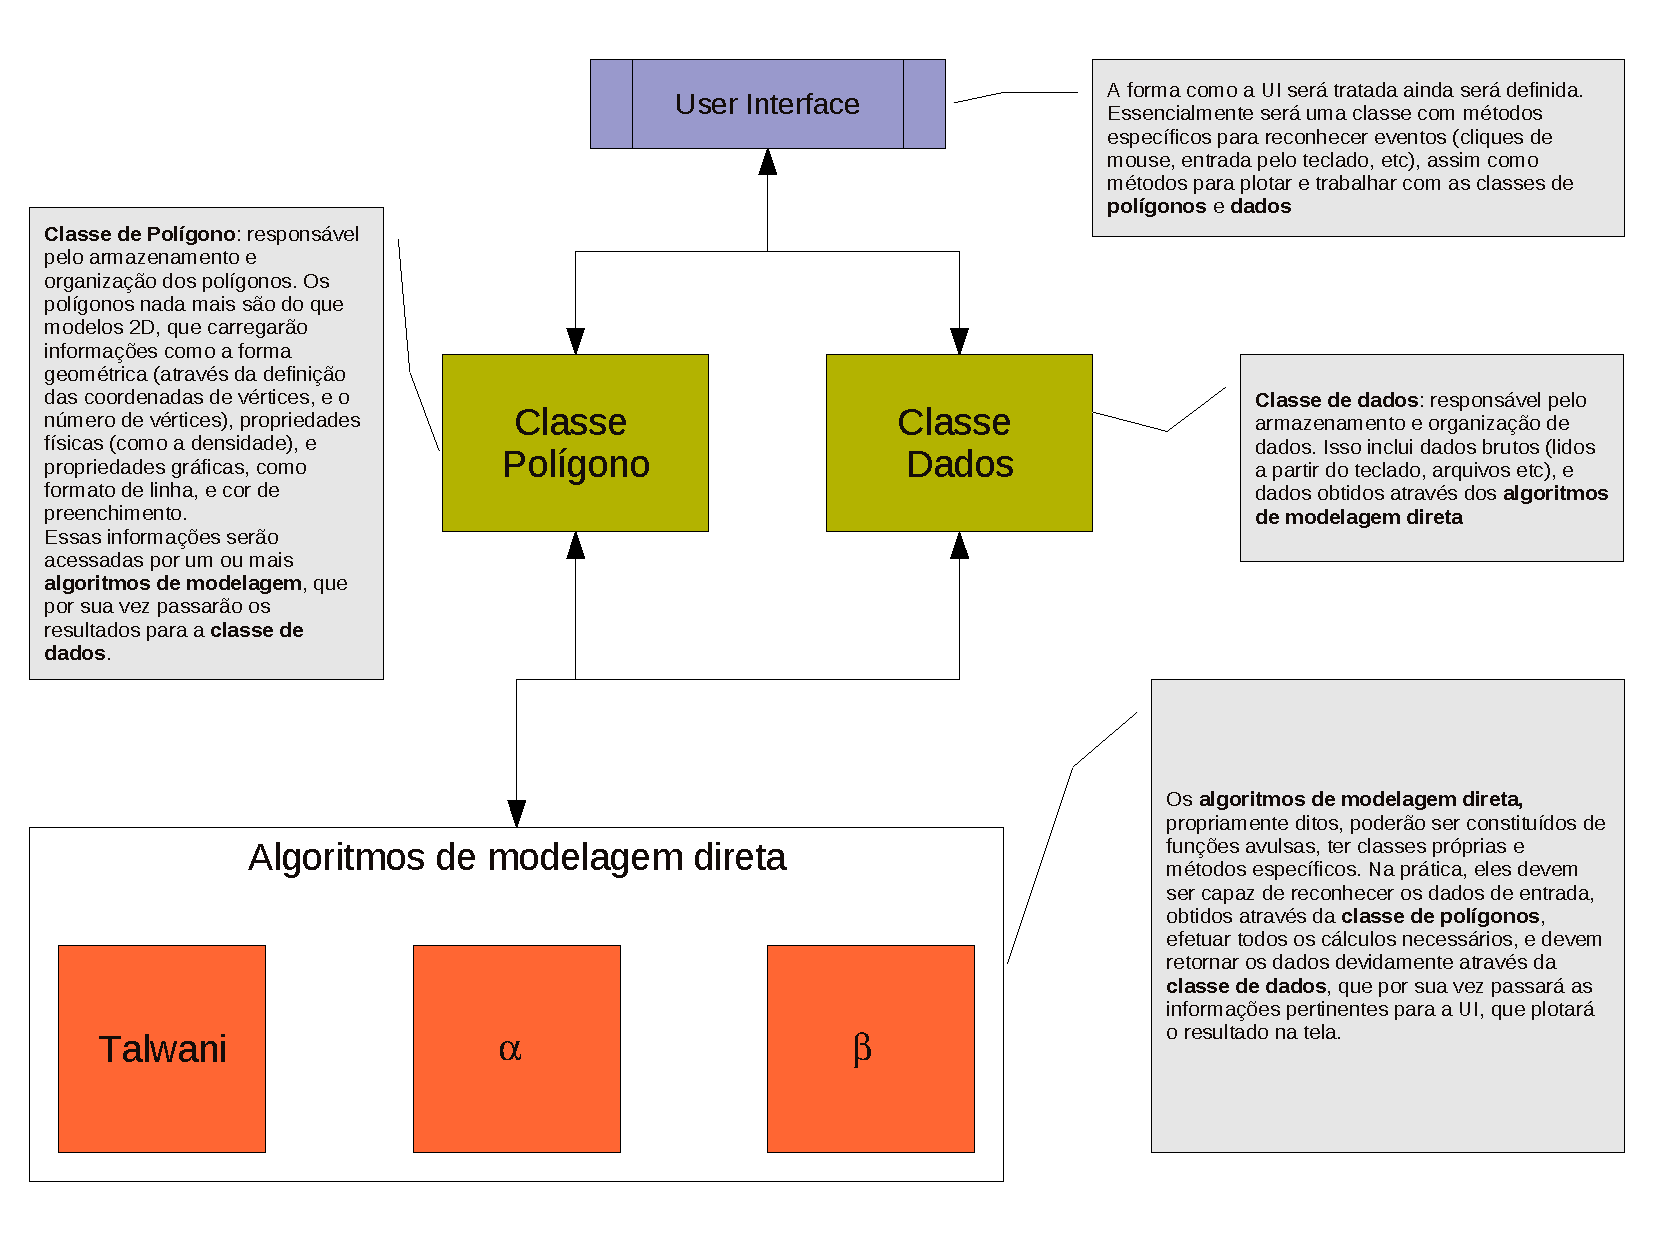
\includegraphics[width=\linewidth]{figs/fluxo-simples.pdf}
    \caption{
        Diagrama de flujo para la primera implementación de un software para el
        modelado gravimétrico de polígonos 2D
        (circa 2009).
    }
    \label{fig:talwani-idea}
\end{figure}

En paralelo, y como proyecto final de su Bachillerato, Leonardo Uieda realiza
una implementación en Python del algoritmo para el cálculo de campos
gravitacionales de tesseroides mediante la \ac{GLQ}.
Luego de reescribirlo en C, este proyecto deriva en el lanzamiento del software
Tesseroids \citep{uieda2016} que ha sido ampliamente utilizado por la comunidad
geocientista.

El éxito de estos proyectos los llevó a aspirar a una idea mucho más
ambiciosa: desarrollar un software de código abierto para modelar el planeta
Tierra de
forma completa.
En ese entonces surge un nombre para el proyecto: \emph{Fatiando a Terra}, que
puede traducirse como \emph{rebanando la Tierra}.

Durante su Master en Geofisica en el Observatório Nacional, Rio de Janeiro,
Leonardo comienza el desarrollo de Fatiando a Terra, transformándolo en el
hogar de las implementaciones que realiza a lo largo de sus investigaciones,
todas mediante el lenguaje Python.
Entre ellas podemos encontrar: modelados directos con diferentes geometrías,
continuación ascendente, deconvolución de Euler, fuentes equivalentes, hasta un
incipiente \emph{framework} de inversión y algunas implementaciones de
tomografías sísmicas simples.

En los años posteriores, cuando la mayoría de los gestores del proyecto se
encontraban cursando sus Doctorados, Fatiando a Terra comienza a cobrar mayor
forma.
Leonardo y Vanderei deciden utilizar el \emph{framework} de inversión para dar
un curso sobre inversiones geofísicas en la Universidade de São Paulo%
\footnote{\url{https://github.com/pinga-lab/inversao-iag-2012}}.
Fatiando adquiere su propio dominio
(\href{https://www.fatiando.org}{fatiando.org}) y su primera página web,
alojada en un servidor casero por José Caparica Jr\footnote{%
    Más adelante se utilizarán los servicios de
    \href{https://readthedocs.org/}{Read The Docs} para alojar el sitio web,
    que más tarde se reemplazarían por GitHub Pages.
}.
Además se elige distribuirlo bajo la licencia
\href{https://opensource.org/licenses/BSD-3-Clause}{BSD 3-clause}.
En 2013, el proyecto es presentado en una charla en SciPy 2013
\citep{uieda2013}.

En los años posteriores el proyecto comienza a cobrar mayor reconocimiento.
Empieza a ser utilizado en publicaciones científicas
\citep[][entre otros]{%
    uieda2012,
    carlos2014,
    oliveira2015,
    hidalgogato2015,
    carlos2016,
    reis2016,
    uieda2017,
    hidalgogato2017,
    siqueira2017%
},
% fill in more papers if you know about some others
dictado de clases
(Tópicos de inversão em
geofísica\footnote{%
    \url{https://www.leouieda.com/teaching/inversao-iag-2012.html}
    y \url{https://www.leouieda.com/teaching/inversao-unb-2014.html}
},
\citet{uieda2014},
Geofísica 1: Gravimetria e magnetometria\footnote{%
    \url{https://www.leouieda.com/teaching/geofisica1.html}
},
Geofísica 2: Sismologia e sísmica\footnote{%
    \url{https://www.leouieda.com/teaching/geofisica2.html}
})
y en trabajos finales de grado y posgrado
\citep{carlos2013, sales2014, soler2015, uieda2016b, melo2020}.
Además comienza a atraer la atención de la comunidad internacional, recibiendo
colaboraciones de investigadores y desarrolladores de diferentes partes del
mundo.
La utilización de la librería \texttt{fatiando} por otros investigadores
e investigadoras deriva a su vez en un ciclo de retroalimentación: quienes
comienzan siendo usuarios, terminan contribuyendo al proyecto.
De esta forma \texttt{fatiando} comienza a alojar implementaciones de métodos
novedosos recientemente publicados \citep{uieda2012b, oliveira2013}.

Mi primea contribución al proyecto consistió en una implementación del promedio
radial del espectro de frecuencias de grillas de gravedad
o magnetismo\footnote{%
    \url{https://github.com/fatiando/fatiando/pull/303}
}.
Desde entonces comencé a involucrarme cada vez más, lo que me permitió adquirir
mayores conocimientos en el uso de controladores de versiones, flujos de
trabajo para el desarrollo colaborativo, creación de funciones de
\emph{testing}, buenas prácticas para el diseño de algoritmos y la importancia
de mantener la documentación actualizada.

La última versión del paquete \texttt{fatiando} es la v0.5, lanzada en
Noviembre de 2016.
Si bien ese paquete en particular se encuentra obsoleto y no recibe mayor
mantenimiento, esto no significa que la vida de el proyecto haya finalizado en
ese entonces.

A partir de 2018 el proyecto tomó una nueva dirección.
El panorama de software de código abierto para Geofísica había cambiado mucho
desde los inicios de Fatiando a Terra: la cantidad de nuevos paquetes diseñados
para atacar diversos problemas de las geociencias había aumentado
considerablemente
\citep{cockett2015, ruecker2017, varga2019, obspy2019}.
Dentro de este nuevo ecosistema, \texttt{fatiando} no poseía un objetivo claro.
Esto no solo hacía difícil que potenciales usuarios y usuarias identifiquen el
propósito del proyecto, sino que también constituía una base de código difícil
de mantener.
Por otro lado, para ese entonces \texttt{fatiando} había sido el hogar de
implementaciones de métodos clásicos de la geofísica, métodos muy novedosos
(orientados principalmente a la investigación científica), así como de código
\emph{juguete} diseñado para ser utilizado en clases para fines didácticos
pero sin las capacidades para atacar problemas reales.
Sumado a esto, la versión de Python 2.7 llegaba pronto a su final de vida, lo
que hacía necesario adaptar \texttt{fatiando} al nuevo Python 3.

Estas razones ponían en evidencia la necesidad de establecer objetivos claros
para el proyecto, así como también repensar su diseño y sustentabilidad
a futuro.
Por esto se tomó la decisión de dividir el proyecto en varios paquetes que
posean objetivos claros y concisos.
Esto permitiría no sólo una fácil adopción por parte de usuarios y usuarias,
sino también que otros proyectos los utilicen como dependencias en caso de
desearlo.
Además, manteniendo los campos de acción de cada paquete aislados del resto,
se facilitaría el desarrollo a futuro: los colaboradores no necesitan
familiarizarse con el proyecto completo, sino solo con algunas de sus partes.
Por otro lado, la decisión de reescribir gran parte del código se presentó como
una oportunidad para pensar mejores diseños del software ya existente y de
implementar mejores
prácticas para el desarrollo de software, estableciendo estándares de calidad
más altos.


\section{Paquetes de software}

Actualmente Fatiando a Terra está compuesto por cuatro paquetes de software
destinados a ofrecer soluciones a diversas problemáticas en geociencias, así
como también a otras áreas de la ciencia:

\begin{description}
    \item[Verde]{%
        Procesado y grillado de datos espaciales
    }
    \item[Boule]{%
        Elipsoides de referencia para aplicaciones geodésicas y geofísicas
    }
    \item[Harmonica]{%
        Procesado, modelado directo e inverso de datos gravimétricos
        y magnéticos
    }
    \item[Pooch]{%
        Descargar y almacenar datos científicos de la web de forma sencilla
    }
\end{description}

\subsection{Verde}

Verde ofrece herramientas para procesar datos espaciales (tales como
muestras geofísicas obtenidas en el campo, mediciones de batimetría, etc)
e interpolarlos sobre grillas regulares.

La mayoría de los muestreos de datos espaciales se componen por datos
irregularmente distribuidos sobre la zona de estudio:
puntos dispersos, trayectos irregulares o líneas casi rectas.
Sin embargo, muchas metodologías de procesado e interpretación requieren que
los datos se sitúen sobre puntos pertenecientes a una grilla regular.
Este problema suele resolverse mediante la interpolación de los datos
originales sobre una grilla regular, proceso que se conoce como
\emph{grillado}.

Dentro de los algoritmos de grillado existe una categoría que se conoce como
\emph{interpolaciones con funciones de base radial} (\emph{radial basis
function interpolation} en inglés) \citep{franke1982}.
Un ejemplo de un algoritmo que entra en esta categoría son las \emph{splines}
biharmónicas \citep{sandwell1987}.
Estos métodos asumen que podemos representar los datos observados por una
combinación lineal de funciones de Green, es decir:

\begin{equation}
    d_i = \sum_{j=1}^M c_j G(\mathbf{p}_i, \mathbf{q}_j),
\end{equation}

\noindent donde $d_i$ es el dato $i$-ésimo, $\mathbf{p}_i$ es la ubicación de
ese mismo punto, $c_j$ es un coeficiente escalar, $G$ es una función de Green y
$\mathbf{q}_j$ es la ubicación del punto que define la función de Green en el
término $j$-ésimo.
El proceso de interpolación consiste en ajustar los valores de los
coeficientes $c_j$ mediante mínimos cuadrados de forma tal que se recuperen los
datos observados, y luego utilizarlos para predecir valores sobre los puntos de
la grilla:

\begin{equation}
    d(\mathbf{p}) = \sum_{j=1}^M c_j G(\mathbf{p}, \mathbf{q}_j),
\end{equation}

\noindent donde $\mathbf{p}$ es la ubicación de cualquier punto de la grilla.

Dentro de Verde hallamos implementaciones de algoritmos de interpolación
de este tipo siguiendo un diseño similar
a los modelos de aprendizaje automático de \emph{scikit-learn}
\citep{sklearn2011}. Esto permite que quienes estén familiarizados con la
aplicación de métodos de aprendizaje automático en Python puedan fácilmente
entender cómo utilizar la \ac{API} de Verde.
Entre los algoritmos de interpolación que se encuentran implementados están las
\emph{splines} biharmónicas, así como métodos más complejos como la
interpolación de vectores 2D con funciones de Green \citep{sandwell2016}.

Como hemos mencionado anteriormente, los interpoladores presentes en
Verde han sido implementados mediante clases que reproducen un
comportamiento similar a las clases de \emph{scikit-learn}.
Los interpoladores en Verde poseen un método \texttt{fit()} que se usa para
ajustar los parámetros $c_j$ mediante mínimos cuadrados partiendo de un
conjunto de datos y sus ubicaciones. Luego podemos hacer uso del método
\texttt{predict()} para predecir valores en cualquier conjunto de puntos,
o bien usando el método \texttt{grid()} podemos predecir sobre una grilla
regular.

Además, Verde cuenta con utilidades para realizar reducciones por
bloque, una clases para determinación de tendencias polinomiales, funciones
para el manejo de coordenadas, y herramientas para realizar validaciones
cruzadas y selección de modelos.

El diseño de Verde permite su extensibilidad: todos los interpoladores
heredan su estructura a partir de una clase base denominada
\texttt{BaseGridder}, lo cual permite construir nuevos tipos de
interpoladores de manera sencilla, restando que definir únicamente el tipo de
función de Green a utilizar.
Además, debido a la compatibilidad con las librerías científicas de Python, es
posible integrarlo a flujos de trabajos establecidos con gran facilidad.

La versión v1.0.0 de Verde ha sido publicada en el Journal of Open
Source Software luego de un proceso abierto de revisión por pares
\citep{verde2018}.
Podemos acceder a la documentación correspondiente a la última versión estable
de la librería en \href{https://www.fatiando.org/verde}{fatiando.org/verde}.


\subsection{Boule}
\label{sec:boule}

Boule es una librería que nos permite representar elipsoides de
referencia mediante objetos. Además nos ofrece herramientas para calcular los
campos gravitatorios que estos elipsoides generan y realizar conversiones
de coordenadas.

Como hemos visto en la sección~\ref{sec:gravedad-terrestre}, un elipsoide de
referencia puede definirse mediante los semiejes mayor $a$ y menor $b$, su masa
total $M$ y su velocidad angular $\omega$.
De forma alternativa pero equivalente, es posible definirlo mediante los
siguientes parámetros:

\begin{itemize}
    \item el semieje mayor $a$,
    \item el achatamiento $f = (a - b) / a$,
    \item la constante gravitacional geocéntrica $GM$ (donde $M$ es la masa
        del elipsoide y $G$ la constante de gravitación universal),
    \item y la velocidad angular $\omega$.
\end{itemize}

Las funcionalidades principales de Boule vienen dadas dentro de las clases
\texttt{Ellipsoids} y \texttt{Sphere}, las cuales nos permiten definir
cualquier elipsoide referencia a partir de los parámetros mencionados.
La clase \texttt{Sphere} está orientada a representar esferas, las cuales
poseen achatamiento nulo y en vez de especificar su semieje mayor, se define su
radio.
A modo de ejemplo, uno podría definir el elipsoide WGS84 como se muestra en le
Código~\ref{lst:boule-wgs84}.
Sin embargo, Boule ya ofrece algunos de los elipsoides de referencia más
ampliamente usados en geodesia y geofísica, tales como el WGS84
(\texttt{boule.WGS84}), el GRS80: Geodetic Reference System
(\texttt{boule.GRS80}) e incluso un elipsoide de referencia para el planeta
Marte definido según los parámetros disponibles en \citet{ardalan2009}
(\texttt{boule.MARS}).
Además podemos hallar elipsoides esféricos para la Luna (\texttt{boule.MOON}),
Venus (\texttt{boule.VENUS}) y Mercurio (\texttt{boule.MERCURY}) definidos
según \citet{wieczorek2015}.

\lstinputlisting[
    float,
    language=Python,
    caption={Ejemplo de definición de elipsoide de referencia con Boule},
    label=lst:boule-wgs84
]{fatiando-examples/boule-wgs84.py}

A su vez, la clase \texttt{Ellipsoids} posee una serie de propiedades que se
calculan a partir de los parámetros que definen cada elipsoide, entre ellos: el
semieje menor $b$, la primera y segunda excentricidad, la excentricidad lineal,
el radio medio del elipsoide (medido desde un sistema geocéntrico), el módulo
del vector aceleración de la gravedad sobre cualquier punto en el ecuador o en
sus polos.
Además, la misma clase ofrece un conjunto de métodos útiles para realizar
cálculos acerca de los campos gravitatorios que genera el elipsoide
y conversión de unidades.
El método \texttt{geocentric\_radius()} nos permite calcular la distancia entre
el centro del elipsoide y cualquier punto de su superficie a partir de su
latitud geodésica o geocéntrica.
Los métodos \texttt{geodetic\_to\_spherical()}
y \texttt{spherical\_to\_geodetic()} nos permiten convertir coordenadas
geodésicas en esféricas geocéntricas o viceversa siguiendo las ecuaciones de
\citet{vermeille2002}.
El método \texttt{normal\_gravity()} implementa la \emph{fórmula cerrada} de
\citet{li2001a} para calcular el módulo de la aceleración de la gravedad
generada por el elipsoide en cualquier punto dado por sus coordenadas
geodésicas.
En el caso de la clase \texttt{Sphere}, su método \texttt{normal\_gravity()}
hace uso de una ecuación más sencilla \citep{heiskanen1967}:

\begin{equation}
    \gamma(\phi, h) =
        \sqrt{\left( \frac{GM}{(R + h)^2} \right)^2
        + \left(\omega^2 (R + h) - 2\frac{GM}{(R + h)^2} \right)
        \omega^2 (R + h) \cos^2 \phi},
\end{equation}

\noindent donde $R$ es el radio de la esfera, $\phi$ la coordenada latitudinal
y $h$ la altitud sobre la superficie de la esfera correspondientes al punto de
observación.

Si bien Boule es una librería que se encuentra en un estado funcional
y puede ser utilizada en investigaciones científicas al día de la fecha, aún no
ha alcanzado su primera versión estable.
Es posible que aún sea necesario realizar modificaciones sobre su diseño en los
planes de incorporar otros tipos de elipsoides, como elipsoides
triaxiales.
Podemos acceder a la documentación correspondiente a la última versión en
\href{https://www.fatiando.org/boule}{fatiando.org/boule}.


\subsection{Harmonica}
\label{sec:harmonica}

Harmonica fue creada con la intención de ser el nuevo hogar de aquellas
implementaciones de métodos de procesamiento y modelado de datos gravimétricos
y magnéticos.
Además, surgió como oportunidad de rediseñar algunas de estas implementaciones
con el objetivo de facilitar su utilización, extensibilidad y mantenimiento
a futuro.

Una de las principales herramientas que ofrece Harmonica son las
funciones de modelado directo para distintas geometrías y para diferentes
sistemas de coordenadas.
La geometría más sencilla que hallamos son masas puntuales en coordenadas
esféricas geocéntricas o en coordenadas Cartesianas, implementando las
ecuaciones~\ref{eq:potencial-masa-puntual} y \ref{eq:gz-particula}.
Podemos calcular los campos gravitacionales producidos por masas puntuales
mediante la función \texttt{point\_mass\_gravity()}.
El Código~\ref{lst:harmonica-point-mass} ejemplifica cómo podemos utilizar esta
función para calcular la aceleración de la gravedad producida por dos masas
puntuales dadas en coordenadas Cartesianas.

Harmonica cuenta con una implementación del método de \citet{nagy2000} para
calcular los campos gravitacionales de prismas rectangulares mediante la
función \texttt{prism\_gravtiy()}, haciendo uso de las correcciones de
\citet{fukushima2020} descriptas en la sección~\ref{sec:prismas-rectangulares}.

La librería también cuenta con una implementación en Python de los algoritmos
de discretización adaptativa y \ac{GLQ} para calcular los campos
gravitacionales de tesseroides con densidad constante, a los cuales podemos
acceder mediante la función \texttt{tesseroid\_gravity()}.

\lstinputlisting[
    float,
    floatplacement=t,
    language=Python,
    caption={%
        Ejemplo de cálculo de aceleración de la gravedad producida por dos
        masas puntuales dadas en coordenadas Cartesianas mediante
        Harmonica.
    },
    label=lst:harmonica-point-mass
]{fatiando-examples/harmonica-point-mass.py}

Cada una de estas funciones admiten una cantidad arbitraria de geometrías
y puntos de observación que pueden venir dadas por estructuras de datos muy
sencillas, tales como listas, tuplas o arreglos de valores numéricos.
Sin embargo pueden ser utilizadas para aumentar el grado de abstracción del
modelo.
Por ejemplo, la función \texttt{prism\_layer()} permite construir una capa de
prismas rectangulares de iguales dimensiones horizontales, distribuidos
regularmente de forma tal que las caras de prismas contiguos se encuentran en
contacto.
La función permite asignar diferentes valores para las caras superiores
e inferiores de los prismas, y devuelve una instancia de
\texttt{xarray.Dataset} que contiene las coordenadas de los centros de los
prismas junto con las coordenadas \texttt{top} y \texttt{bottom} para cada uno
de ellos.
Harmonica ofrece un \emph{accessor} de Xarray para poder calcular los campos
gravitatorios que toda la capa genera sobre un conjunto de puntos de
observación, la cual hace uso de función \texttt{prism\_gravity()} mencionada
anteriormente.
Este tipo de capas resultan muy útiles para calcular los efectos gravimétricos
de la topografía o para realizar inversiones como las de \citet{uieda2017}.
El Código~\ref{lst:harmonica-prism-layer} ejemplifica cómo podemos usar la
función \texttt{prism\_layer()} junto con el método \texttt{prism\_gravity()}
del \emph{accessor} para calcular el efecto gravitatorio de la topografía de
Sudáfrica sobre una grilla regular a 4000\m{} de altitud.

\lstinputlisting[
    float,
    floatplacement=p,
    language=Python,
    caption={%
        Ejemplo de cálculo de efecto gravitatorio de la topografía de Sudáfrica
        sobre una grilla regular haciendo uso de
        \texttt{harmonica.prism\_gravity()}.
    },
    label=lst:harmonica-prism-layer
]{fatiando-examples/harmonica-prism-layer.py}

La mayoría de los métodos de modelado directo involucran cómputos moderadamente
complejos, los cuales pueden conllevar a un alto costo computacional,
especialmente a la hora de modelar grandes cantidades de geometrías sobre
muchos puntos de observación.
Escribir estas funciones en Python puro resultaría en implementaciones que no
harían un uso eficiente de los recursos computacionales debido a la misma
naturaleza del interprete de Python.
Las alternativas más viables son recurrir a código precompilado (escribiendo
las implementaciones en lenguajes como C o FORTRAN y luego añadir
\emph{wrappers} de Python) o bien a compilaciones en tiempo de ejecución.
En los orígenes de de Harmonica, hemos optado por realizar nuestras
implementaciones mediante Numba \citep{numba2015}: un compilador de Python de
alto desempeño.
Numba se encarga de precompilar el código que implementa cada uno de estos
algoritmos al momento de ejecutar las funciones por primera vez, utilizando en
adelante los binarios ya compilados.
Mediante este método no solo podemos hacer un uso mucho más eficiente de los
recursos computacionales sino que además podemos habilitar sencillamente la
paralelización de nuestros algoritmos, distribuyendo la tarea en los
núcleos disponibles del procesador donde se está ejecutando.
Además, dada la naturaleza de Numba, no es necesario que distribuyamos los
binarios de Harmonica para cada plataforma o sistema operativo: Numba se
encarga de la precompilación durante el tiempo de ejecución.
De esta manera, se simplifica mucho la tarea de distribuir e instalar
Harmonica en cualquier tipo de plataforma.

Otra de las capacidades que presenta Harmonica es la de realizar cálculos
a partir de los algoritmos de fuentes equivalentes.
La clase \texttt{EquivalentSources} contiene una implementación del método de
fuentes equivalentes que utiliza fuentes puntuales y la inversa de la distancia
como función de Green (tal y como se describe en la
sección~\ref{sec:equivalent-sources-technique}).
El ajuste de los coeficientes de las fuentes se realiza mediante un algoritmo
de mínimos cuadrados amortiguados, haciendo uso del parámetro de
\emph{amortiguamiento} adimensional introducido en la
sección~\ref{sec:eql_inversion}.
\texttt{EquivalentSources} permite ajustar fuentes equivalentes dadas en
coordenadas Cartesianas, mientras que \texttt{EquivalentSourcesSph} nos permite
aplicar la misma metodología pero definiendo las fuentes puntuales y los puntos
de observación en coordenadas esféricas geocéntricas.
Estas clases heredan muchos de los métodos y atributos de la clase
\texttt{BaseGridder} de Verde, haciendo que su utilización sea a su vez
muy similar a la que encontramos en los métodos de aprendizaje automático de
scikit-learn \citep{sklearn2011}.
Las decisiones de diseño han permitido que los métodos de
\texttt{EquivalentSources} y \texttt{EquivalentSourcesSph} reutilicen muchas de
las funciones centrales del modelado directo de masas puntuales, permitiendo no
solo un ahorro en cantidad de código, sino también el reciclado de las
oportunidades que estas proveen mediante el compilador Numba, como paralelizar
la construcción de la matriz Jacobiana.

Harmonica ofrece además algunas otras funcionalidades para procesar datos
gravimétricos: aplicación de la corrección de Bouguer utilizando una
aproximación de placa infinita, cálculo de profundidad de raíces según un
modelo isostático de Airy, la capacidad de leer archivos \texttt{.gdf}
provistos por el servicio
ICGEM\footnote{\url{http://icgem.gfz-potsdam.de/home}}, creación de muestras
sintéticas aéreas o sobre terreno a partir de muestras reales.

Si bien Harmonica es una librería que se encuentra en un estado funcional
y puede ser utilizada en investigaciones científicas al día de la fecha, aún no
ha alcanzado su primera versión estable.
Podemos acceder a la documentación correspondiente a la última versión en
\href{https://www.fatiando.org/harmonica}{fatiando.org/harmonica}.

% Planes a futuro:

% incluir gradient-boosted eqls y variable density tesseroids

% derivadas espaciales de grillas (verticales con FFT)

% Euler deconvolution

% inversion: nuevo framework de inversion

\subsection{Pooch}

Muchas de las librerías de software científico hacen uso de datos de muestra
para ejemplificar su funcionamiento en las secciones de la documentación que se
conocen como \emph{Galería de ejemplos}.
Usualmente estos datos de muestra se incluyen dentro de los repositorios donde
se aloja el mismo código fuente de la librería, sin embargo estos archivos de
datos no son empaquetados para su distribución con el objetivo de reducir el
tamaño de las futuras instalaciones.
En cambio, los datos de muestra suelen ser descargados al ser necesarios
mediante código implementado dentro de cada una de estas librerías, haciendo
uso de paquetes de Python para descargar archivos mediante protocolo HTTP por
ejemplo.
Pooch surge como una solución a este problema transversal a muchas
librerías del ecosistema científico de Python.

\lstinputlisting[
    float,
    floatplacement=h,
    language=Python,
    caption={%
        Ejemplo de descarga de archivos con Pooch mediante la
        clase \texttt{pooch.Pooch}. Este código es a modo de ejemplificación
        y no está escrito para ser ejecutado.
    },
    label=lst:pooch-registry
]{fatiando-examples/pooch-registry.py}


Pooch permite gestionar un \emph{registro} en el cual podemos listar las
direcciones de cada uno de los archivos que queremos ofrecer para su descarga,
junto con el \emph{hash} de una suma de verificación. Al solicitar algún
o algunos de estos archivos, Pooch se encarga de descargarlos de su
correspondiente localización, almacenarlos en un \emph{caché} local y realizar
una suma de verificación con el objetivo de certificar la integridad de los
mismos.
La descarga de los archivos se lleva a cabo únicamente si no existe tal archivo
en el \emph{caché} local.
En el Código~\ref{lst:pooch-registry} podemos visualizar cómo es posible
utilizar la función \texttt{pooch.create()} para inicializar una instancia de
la clase \texttt{pooch.Pooch}, especificando el directorio donde se descargarán
los archivos, la dirección base donde se encuentran alojados los archivos de
interés, y el \emph{registro} donde enumeramos el nombre de los archivos y sus
\emph{hashes} de las sumas de verificación.
Luego podemos solicitar la descarga de uno de los archivos mediante el método
\texttt{fetch()}, el cual devuelve la ruta al archivo descargado y almacenado
localmente.

Pooch no sólo nos permite descargar archivos desde el protocolo HTTPS,
sino también desde FTP y SFTP con autenticación.
Incluso es posible descargar archivos almacenados en repositorios de acceso
abierto como Zenodo\footnote{\url{https://zenodo.org/}}
o figshare\footnote{\url{https://figshare.com}} únicamente mediante el
\ac{DOI}.
A su vez, también soporta diferentes tipos de suma de verificación, como
SHA256, MD5, XXH128, entre otras.
Además ofrece la posibilidad de realizar postprocesados luego de la descarga,
como por ejemplo descomprimir archivos \texttt{.zip}, \texttt{.tar},
\texttt{.gzip}, \texttt{.xz}, etc.

El paquete presenta ciertas cualidades que lo hacen un excelente candidato para
ser utilizado por librerías de terceros.
En primer lugar, es posible configurarlo para que se adapte a diferentes
necesidades en pocas líneas con una sintaxis sencilla.
En segundo lugar, es un paquete puramente escrito en Python con dependencias
mínimas.
Y por último, presenta un alto grado de extensibilidad: es posible definir
funciones propias para otro tipos de descargas (mediante otros protocolos, por
ejemplo) o bien para realizar postprocesados. Estas funciones personalizadas
puede acoplarse fácilmente al \emph{framework} de Pooch, permitiendo
utilizar su misma sintaxis y sus capacidades de descarga, almacenamiento
y comprobación de sumas de verificación, incluso en aplicaciones particulares.

La versión v0.7.1 de Pooch fue publicada en el Journal of Open Source
Software luego de una revisión abierta por pares \citep{pooch2020}.

\lstinputlisting[
    float,
    language=Python,
    caption={%
        Ejemplo de descarga de archivos con Pooch mediante la
        función \texttt{pooch.retrieve()}.
    },
    label=lst:pooch-retrieve
]{fatiando-examples/pooch-retrieve.py}

Hasta entonces la principal audiencia de Pooch consistía en otros
desarrolladores de software que deseaban una forma sencilla de distribuir datos
de muestra a sus usuarios.
Sin embargo, en los meses subsiguientes se presentó la oportunidad de incluir
otro tipo de audiencia al paquete: usuarios finales que deseaban descargar
pocos archivos por única vez.
Esto se materializó con la creación de la función \texttt{pooch.retrieve()} que
permite acceder a las mismas funcionalidades de Pooch, pero sin la
necesidad de predefinir una instancia de \texttt{pooch.Pooch} y con una
interfaz más sencilla.
El Código~\ref{lst:pooch-retrieve} ejemplifica cómo podemos utilizar la función
\texttt{pooch.retrieve()} para descargar un archivo, almacenarlo localmente
y comprobar su suma de verificación en una única ejecución.
La función devuelve la ruta al archivo descargado y almacenado localmente.

Actualmente Pooch es utilizado por varias librerías del ambiente
científico, entre ellas: MetPy \citep{metpy}, icepack \citep{icepack}, MOABB
\citep{moabb}, MNE-Python \citep{mnepython}, yt \citep{yt2010} junto a otras
librerías de Fatiando como Harmonica y Verde.
Además, proyectos con aplicaciones más amplias han incluido a Pooch
dentro de sus dependencias, como Xarray \citep{xarray2017}, scikit-image
\citep{skimage} y Project Pythia\footnote{\url{https://projectpythia.org/}}.

La documentación correspondiente a la última versión estable de Pooch
puede hallarse en \href{https://www.fatiando.org/pooch}{fatiando.org/pooch}.


\section{Desarrollo y mejores prácticas}
\label{sec:best-practices}

Desde sus orígenes, Fatiando a Terra ha sido desarrollado siguiendo las mejores
prácticas que se encontraban en conocimiento de sus desarrolladores.
Es por esta razón que a lo largo de sus años de vida se hayan incorporado cada
vez mayor cantidad o mejores herramientas para desempeñar estas mejores
prácticas, a medida que los desarrolladores adquirían mayores conocimientos.

Todo desarrollo dentro del proyecto se realiza mediante un software de
controlador de versiones, y a excepción de algunos momentos en la concepción
del proyecto, utilizamos \texttt{git}\footnote{\url{https://git-scm.com}} como
controlador de versiones distribuido
y GitHub\footnote{\url{https://www.github.com}} como servidor de repositorios.

Gracias a \texttt{git}, cada librería posee una \emph{rama} principal de
desarrollo donde se provee del código fuente que será utilizado por los
usuarios y usuarias finales.
El flujo de desarrollo de cada una de las librerías del proyecto se basa en los
\emph{Issues} y \emph{Pull Requests} que ofrece GitHub.
En cada \emph{Issue} ponemos en evidencia la existencia de un problema en el
código de la \emph{rama} principal, exponemos una nueva idea a implementar
a futuro o solicitamos una nueva capacidad o comportamiento del código
existente.
Los \emph{Issues} representan un canal de comunicación entre toda la comunidad,
incluyendo usuarios, desarrolladores y contribuidores.

Cada vez que alguien desea colaborar con alguna modificación o una nueva
implementación, esta persona escribe su código en una nueva \emph{rama} que
se desprende de la principal y abre un \emph{Pull Request}, es decir, una
solicitud a los mantenedores de incluir ese nuevo código en la rama principal.
Dentro de los \emph{Pull Requests} otros colaboradores pueden realizar una
revisión del código, sugerir cambios y discutir alternativas, de forma tal que
la propuesta inicial alcance el estado necesario para poder ser incorporada
al código fuente de la librería.
Los requisitos para que un nuevo código sea aceptado no son estrictos, sin
embargo se busca alcanzar un determinado estándar de calidad siguiendo un
conjunto de mejores prácticas.
Las revisiones de código no tienen como objetivo determinar si una cierta
contribución debe ser aceptada o rechazada, sino que se toman como punto de
partida para aplicar las modificaciones necesarias hasta alcanzar dicho
estándar de calidad.
La guía para los y las
contribuidores%
\footnote{
    \url{https://github.com/fatiando/community/blob/main/CONTRIBUTING.md}%
}
brinda instrucciones detalladas de cómo llevar a cabo este proceso.

Muchas de las mejores prácticas que aplicamos a lo largo del proyecto pueden
hallarse en \citet{wilson2014,wilson2017}, sin embargo presentamos
a continuación una descripción detallada de las más importantes.

\subsection{Estilo de escritura}

El lenguaje Python admite estilos de escritura muy variados, priorizando que el
código sea legible a poseer una sintaxis muy estricta.
Sin embargo, a la hora de mantener una base de código entre muchos
desarrolladores, es recomendable establecer un estilo de escritura común.
Dentro del proyecto hemos decidido seguir los lineamientos establecidos en
PEP8 (siglas en inglés de \emph{Python Enhancement Proposals}: propuestas de
mejoras de Python)\footnote{\url{https://www.python.org/dev/peps/pep-0008/}}.
Dentro de estos lineamientos se establecen recomendaciones acerca del tipo de
\emph{indentación} (sangrado) que se debe utilizar; la cantidad máxima de
caracteres por línea; la cantidad de líneas vacías antes y después de la
definición de funciones, clases y métodos; la forma en que se deben nombrar las
variables, las funciones y las clases; entre muchas otras.

Con el objetivo de facilitar la tarea de adecuar cualquier nuevo código a estas
reglas, tanto para quien lo escribe como para quien lo revisa, hemos
normalizado el uso del auto-formateador
Black\footnote{\url{https://black.readthedocs.io/en/stable/}}, el cual modifica
automáticamente cualquier código sintácticamente correcto para adecuarlo
a muchos de los lineamientos establecidos en PEP8.
De esta forma, los y las contribuidores pueden utilizar el estilo de escritura que
les sea más cómodo y luego correr Black para que adopte el estilo que
utilizamos en Fatiando.

Sin embargo, Black no es capaz de aplicar algunas de las recomendaciones
establecidas en PEP8, especialmente las que tienen que ver con el nombre de las
variables, el modo de uso de operadores lógicos, entre otras.
Para este tipo de situaciones hacemos uso de otro software que permite detectar
este tipo de errores, además de muchas otras recomendaciones para mejorar la
escritura de nuestro código:
\texttt{pylint}\footnote{\url{https://pylint.org/}}.
Esta herramienta no solo identifica violaciones a PEP8, sino que además realiza
un análisis más profundo del código: desde detectar variables definidas pero no
utilizadas, módulos importados innecesariamente, definiciones de funciones
extremadamente largas o con muchos argumentos, entre muchas otras.
Dentro del proyecto utilizamos \texttt{pylint} para identificar este tipo de
errores más difíciles de detectar, sin embargo establecemos un criterio más
flexible: permitimos ignorar alguna de sus recomendaciones si lo consideramos
conveniente.

\subsection{Documentación}

Cada nueva función, clase o método dentro de las librerías de Fatiando debe
estar acompañado de su correspondiente documentación, es decir, un texto que
describa su funcionamiento, que enumere los parámetros de entrada que admite
y que especifique sus salidas o resultados.
Opcionalmente la documentación puede incluir ejemplos sencillos de uso,
mostrando cuáles son las salidas esperadas para el mismo, y referencias
a artículos científicos si el código en cuestión implementa algún método que
podamos hallar en la literatura.

Dentro del proyecto se ha establecido como criterio que la documentación debe
seguir un estilo establecido por
\texttt{numpydoc}\footnote{\url{https://numpydoc.readthedocs.io/}},
una extensión para Sphinx\footnote{\url{https://www.sphinx-doc.org/}}.
Mediante Sphinx podemos generar la documentación de toda la librería como un
sitio web estático que puede ser servido y consultado por los usuarios y las
usuarias.
Como hemos mencionado anteriormente, las documentaciones de todos los paquetes
del proyecto se pueden hallar bajo el dominio
\href{https://www.fatiando.org}{fatiando.org}.

Además de la documentación de cada función, clase o método, Sphinx nos permite
agregar otro tipo de contenido: descripción del paquete, instrucciones
para la instalación, galería de ejemplos, tutoriales específicos para
diferentes tareas, etc.
Toda la documentación de cada uno de los proyectos forma parte del mismo
repositorio sobre el cual desarrollamos el código fuente, lo que nos permite
hacer uso del mismo sistema de control de versiones, \emph{Issues} y \emph{Pull
Requests} para su mantenimiento y actualización.
Esto no solo simplifica la tarea concentrando todo el flujo de trabajo en un
mismo lugar, sino que también permite recibir reportes de mejora de la
documentación existente del mismo modo que lo hacemos con el código.

Una de las mejores prácticas que hemos aplicado dentro del proyecto es la
manera en la que diseñamos el código para una nueva implementación.
En vez de partir por la escritura de la implementación misma, comenzamos por la
creación de sus ejemplos, en donde identificamos de qué manera deseamos que esa
nueva porción de software sea utilizada.
Es decir, partimos nuestro diseño bosquejando la interfaz con la cual los
usuarios y usuarias interactuarán.
Luego procedemos a redactar la documentación de esta nueva implementación,
siendo consistentes con el diseño inicial.
Una vez que nos encontramos conformes con la propuesta, procedemos a escribir
la propia implementación.
Este flujo de trabajo ha demostrado ser más eficiente que otros que guardan el
diseño de la interfaz como última instancia, lo cual suele requerir múltiples
iteraciones entre modificaciones de la implementación y de la interfaz.


\subsection{Pruebas de software}

Una de las mejores prácticas más conocidas para el desarrollo de software
consiste en el agregado de funciones de prueba o \emph{testing} para cada nueva
implementación.
Las funciones de prueba son porciones de software que tienen como único
objetivo corroborar el buen funcionamiento del código que compone un
determinado paquete.
Estas funciones de prueba no están destinadas a ser utilizadas por usuarios
finales de la forma en que sí son diseñadas las funciones incluidas en la
\ac{API} del proyecto.
Por el contrario, se añaden para ser ejecutadas por desarrolladores o por
servicios de integración continua (ver sección~\ref{sec:ci}).

En el caso particular del software científico, un comportamiento no deseado de
nuestro código puede conllevar la obtención de resultados erróneos, que pueden
repercutir en el avance de una determinada disciplina o incluso hasta en la
toma de decisiones sobre sociedades y la vida de personas.
Si bien estos comportamientos erróneos pueden ser percibidos por los usuarios
o desarrolladores durante el uso cotidiano del código, muchos otros pueden
permanecer inadvertidos durante mucho tiempo.
Las pruebas de software son herramientas extremadamente útiles a la hora de
detectar estos comportamientos no deseados, especialmente porque permiten
adelantarse y reconocerlos antes de que puedan tener impactos negativos.
Nos permiten detectar errores mientras escribimos una nueva implementación, al
realizar modificaciones sobre el código existente, o al intentar utilizar
nuestro proyecto con versiones actualizadas de sus dependencias.

Una de las metodologías más aplicadas para construir funciones de prueba son
las \emph{pruebas unitarias} (\emph{unit testing}).
Estas consisten en concebir el código fuente de nuestro proyecto como un
conjunto de unidades independientes de código.
Cada unidad de código puede ser interpretada de forma distinta, pero podemos
asumir que cada función o método es una unidad.
Las pruebas unitarias consisten en escribir funciones de prueba que corroboren
el buen funcionamiento de una unidad a la vez, o al menos un determinado
comportamiento de una única unidad.
Cada una de estas funciones de prueba debe ser independiente del resto y ser
capaz de ser ejecutada de manera automatizada.
Además, es deseable que todas las funciones de pruebas formen un conjunto
completo de prueba, es decir, que las funciones de prueba en su totalidad
corroboren el buen funcionamiento de toda la base de código de la librería.

Dentro de Fatiando a Terra hacemos un uso intensivo de las pruebas de software,
siendo un requerimiento indispensable para que un nuevo código pueda formar
parte de cada paquete.
Para su escritura y ejecución hacemos uso del paquete
\texttt{pytest}\footnote{\url{https://docs.pytest.org}}, del cual se pueden
obtener reportes detallados sobre la ejecución de las funciones de testeo,
identificando cuál o cuáles fallan y por qué razón.
Además, \texttt{pytest} ofrece herramientas muy útiles para una escritura más
simple de estas funciones de prueba, tales como parametrizaciones mediante
decoradores de funciones y la creación de \emph{fixtures} que pueden se
utilizados transversalmente en cada función de testeo, ahorrando la necesidad
de repetir código.
\texttt{pytest} permite además generar un reporte de cobertura, es decir, un
porcentaje de qué cantidad de la base del código es sometida a prueba y
detalla cuáles son las líneas que no.

La gran mayoría del código fuente que podemos encontrar en las librerías del
proyecto son fácilmente probables, especialmente las que tienen que ver con
estructuras de datos y comportamientos particulares frente a diferentes
parámetros.
Sin embargo, en algunas de nuestras librerías incluimos implementaciones de
métodos numéricos y soluciones analíticas a problemas geofísicos, los cuales
pueden presentar determinada complejidad de corroborar, ya que su
implementación surge de la propia necesidad de arribar a los resultados
numéricos que ellas generan.
A pesar de esto, existen algunos métodos para someterlas a prueba.
Tanto las soluciones analíticas como los cálculos numéricos pueden ser
corroborados con valores conocidos o con soluciones analíticas a casos
particulares.
Por ejemplo, la implementación del cálculo de gravedad normal en Boule (ver
sección~\ref{sec:boule}) es corroborada por comparación con la ecuación de
Somigliana (ec.~\ref{eq:somigliana}) sobre puntos en la superficie del
elipsoide.
Así como la implementación del modelado directo por tesseroides en Harmonica
(ver sección~\ref{sec:harmonica}) es puesta a prueba comparando sus resultados
numéricos con la solución analítica para un cascarón esférico.
Otro método consiste en verificar que nuestros resultados numéricos
o analíticos verifican determinadas propiedades matemáticas.
Por ejemplo, la implementación del modelado directo por prismas rectangulares
presente en Harmonica (ver sección~\ref{sec:harmonica}) debe verificar una
determinada simetría: los valores de los campos a lados opuestos del prisma
deben poseer los mismos valores.

Es importante destacar que un conjunto finito de funciones de prueba no
garantizan la inexistencia de comportamientos no deseados o errores en la base
del código, al igual que una cobertura del 100\% no es un indicativo de la
calidad del conjunto de pruebas de software.
Es por esto que es necesario considerar la escritura de funciones de prueba tan
importantes como las implementaciones mismas.


\subsection{Automatización e integración continua}
\label{sec:ci}

Muchas de las tareas involucradas en la aplicación de las mejores prácticas
mencionadas deben ser realizadas repetitivamente ante una nueva solicitud de
incorporación de código o incluso periódicamente tras actualizaciones en las
dependencias de cada librería.
Realizar estas tareas de forma manual no solo representa una rutina tediosa,
sino que además no resulta eficaz.
Es por ello que dentro del proyecto recurrimos a los servicios de
\emph{integración continua} para automatizar muchas de estas tareas,
quitándonos el peso de tener que ejecutarlas manualmente y permitiéndonos
ocupar ese tiempo en otras tareas de forma más eficiente.

Cada vez que un contribuidor crea un \emph{Pull Request}, el servicio de
integración continua que provee GitHub mediante las GitHub Actions realiza
diversas tareas.
Haciendo uso de máquinas virtuales, ejecuta comprobaciones sobre el estilo de
escritura del último código publicado en ese \emph{Pull Request}.
Para ello utiliza tanto Black como \texttt{pylint}, devolviendo un reporte de
su ejecución donde se pueden identificar las violaciones a las recomendaciones
que realizan estas dos utilidades.
Además, mediante otro conjunto de máquinas virtuales procede a instalar el
nuevo código junto con todas sus dependencias bajo diferentes sistemas
operativos y haciendo uso de diferentes versiones de Python 3 (Python 3.7,
Python 3.8, Python 3.9 por ejemplo).
Luego ejecuta la \emph{suite} de pruebas de software en cada configuración
mediante \texttt{pytest}, devolviendo también su reporte de fallos y de
cobertura.
Otro servicio de integración continua que se ejecuta es la construcción de la
documentación correspondiente a este nuevo código, la cual también devuelve
información acerca de posibles fallos que se hayan encontrado.
Dentro de la interfaz del \emph{Pull Request} podemos observar si algunas de
estas ejecuciones han fallado, evitando que incorporemos ese nuevo código en la
\emph{rama} principal.

En cada una de las librerías del proyecto se ha establecido como requisito
mínimo para incorporar un código nuevo a la \emph{rama} principal que:

\begin{itemize}
    \item las comprobaciones de estilos escritura pasen correctamente,
    \item las pruebas de software no presenten errores en ninguna plataforma, y
    \item la documentación pueda construirse sin errores.
\end{itemize}

De esta forma se garantiza que la \emph{rama} principal cuente únicamente con
código que sigue estos estándares, bajo la idea de que es más sencillo
y factible enmendar una contribución antes de ser incorporada que solucionar el
problema posteriormente.

Los servicios de integración continua no son utilizados únicamente durante el
proceso de \emph{Pull Request}.
Las GitHub Actions son usadas además para construir la documentación presente
en la \emph{rama} principal cada vez que un cambio se incorpora a ella
y publicarla de forma automática para que esté disponible para toda la
comunidad.

Otra tarea que se realiza con cierta periodicidad dentro del proyecto es la de
generar \emph{lanzamientos} (\emph{releases} en inglés).
Cada lanzamiento consiste en asignar un número a una versión particular del
código y publicarlo bajo esa denominación en servicios que proveen las fuentes
para distintos gestores de paquetes, tales como
PyPI\footnote{\url{https://pypi.org/}} (\emph{Python package index})
y \texttt{conda-forge}\footnote{\url{https://conda-forge.org/}}.
Gracias a esto los usuarios pueden descargar e instalar nuestras librerías
mediante la utilización de gestores de paquetes.
Por ejemplo, si se desea instalar Boule con el gestor \texttt{pip} es posible
hacerlo ejecutando:

\begin{lstlisting}[language=bash,frame=]
pip install boule
\end{lstlisting}

\noindent Y si deseamos instalar Harmonica con el gestor \texttt{conda} podemos
hacerlo con:

\begin{lstlisting}[language=bash,frame=]
conda install --channel conda-forge harmonica
\end{lstlisting}

Cada vez que se genera un nuevo lanzamiento mediante GitHub,
los servicios de integración continua publican esta nueva versión en PyPI
mediante su \ac{API} de forma automática.
Afortunadamente, \texttt{conda-forge} realiza una tarea similar pero desde su
lado: registra un nuevo lanzamiento en los paquetes que provee y automatiza el
proceso para su publicación.


\section{Comunidad}

Una de las partes fundamentales para que el proyecto se haya podido desarrollar
de la forma en que lo hizo es la comunidad que se ha construido a su alrededor
y las comunidades con las que ésta interactúa.
La comunidad de Fatiando a Terra no solo esta formada por los mantenedores del
código, desarrolladores y contribuidores, sino también por usuarios
y usuarias que intercambian ideas y preguntas mediante los canales de
comunicación que se han establecido.

Hacia el resto de la comunidad científica Fatiando se presenta mediante su
página web, donde se pueden encontrar descripciones de cada una de las
librerías, enlaces a la documentación respectiva de cada una de ellas,
instrucciones de instalación, videos tutoriales, información sobre nuestros
canales de comunicación e instructivos para comenzar a colaborar en el
proyecto.

Como hemos mencionado anteriormente, gran parte del intercambio de ideas al
respecto del desarrollo de cada librería, reportes de fallos, propuesta de
ideas y revisión de código se realiza mediante GitHub.
Sin embargo, muchas otras conversaciones suceden dentro de la sala de
Slack\footnote{\url{http://contact.fatiando.org/}}, donde se realizan
preguntas, se ofrecen soluciones a problemas comunes, se anuncian eventos
y más.
La sala de Slack constituye un canal de comunicación más informal y más
directo entre los integrantes de la comunidad.
Además, se organizan dos tipos de videollamadas periódicas: las reuniones de la
comunidad y las reuniones de desarrolladores.
Las primeras se llevan a cabo un par de veces al año y tienen como objetivo la
sociabilización y la discusión de proyectos, sin entrar en muchos detalles
técnicos.
Las segundas suceden semanalmente y en ellas se discuten problemáticas
específicas del desarrollo de las librerías.
A pesar de la diferente naturaleza de ambas, cualquier persona es bienvenida
a participar, independientemente de su grado de conocimiento o habilidades
técnicas.

Dentro de cada uno de los canales de comunicación de la comunidad se espera
que sus integrantes respeten el Código de
Conducta%
\footnote{%
    \url{https://github.com/fatiando/community/blob/main/CODE_OF_CONDUCT.md}%
}
con el objetivo de generar un ambiente ameno y respetuoso.

% Interacción con otros proyectos?


\section{Adopción en la comunidad científica}

Desde sus comienzos, las herramientas provistas en Fatiando a Terra han sido
utilizadas en publicaciones científicas por investigadores de diferentes partes
del mundo.
Muchas de ellas citan a los artículos \citet{uieda2013} y \citet{verde2018}.
Además, el proyecto ha sido presentado en congresos científicos y reuniones
científicas \citep{uieda2013,uieda2020b,soler2021c}.

\begin{figure}
    \centering
    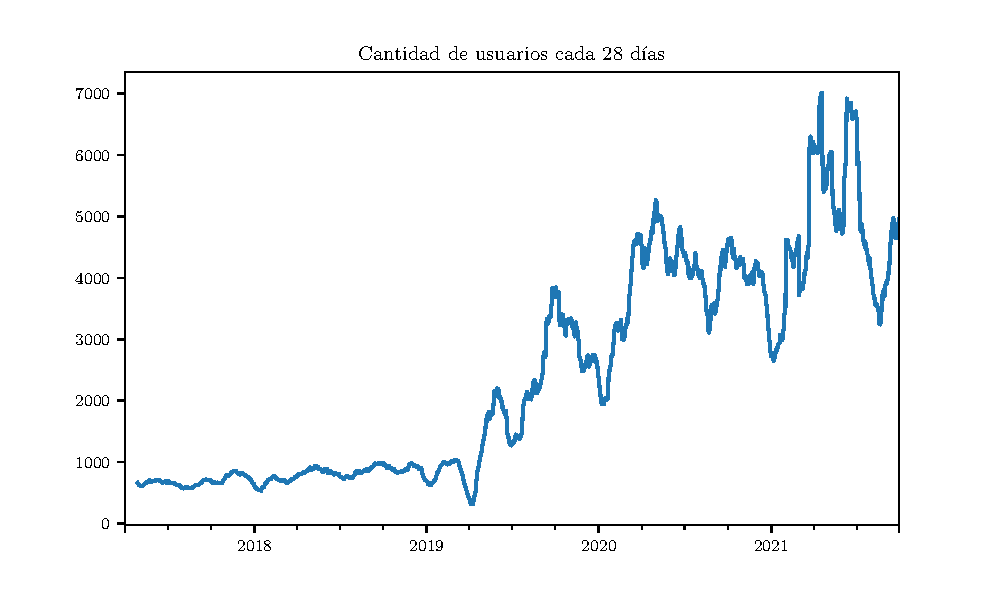
\includegraphics[width=0.7\linewidth]{figs/fatiando/users_history.pdf}
    \caption{
        Cantidad de visitas a \href{https://fatiando.org}{fatiando.org} entre
        Abril de 2017 y Septiembre de 2021 en ventana móvil de 28 días.
        Cada valor representa la cantidad de visitas recibidas en una ventana
        de 28 días centrada en su fecha correspondiente.
    }
    \label{fig:fatiando-users-history}
\end{figure}

\begin{figure}
    \centering
    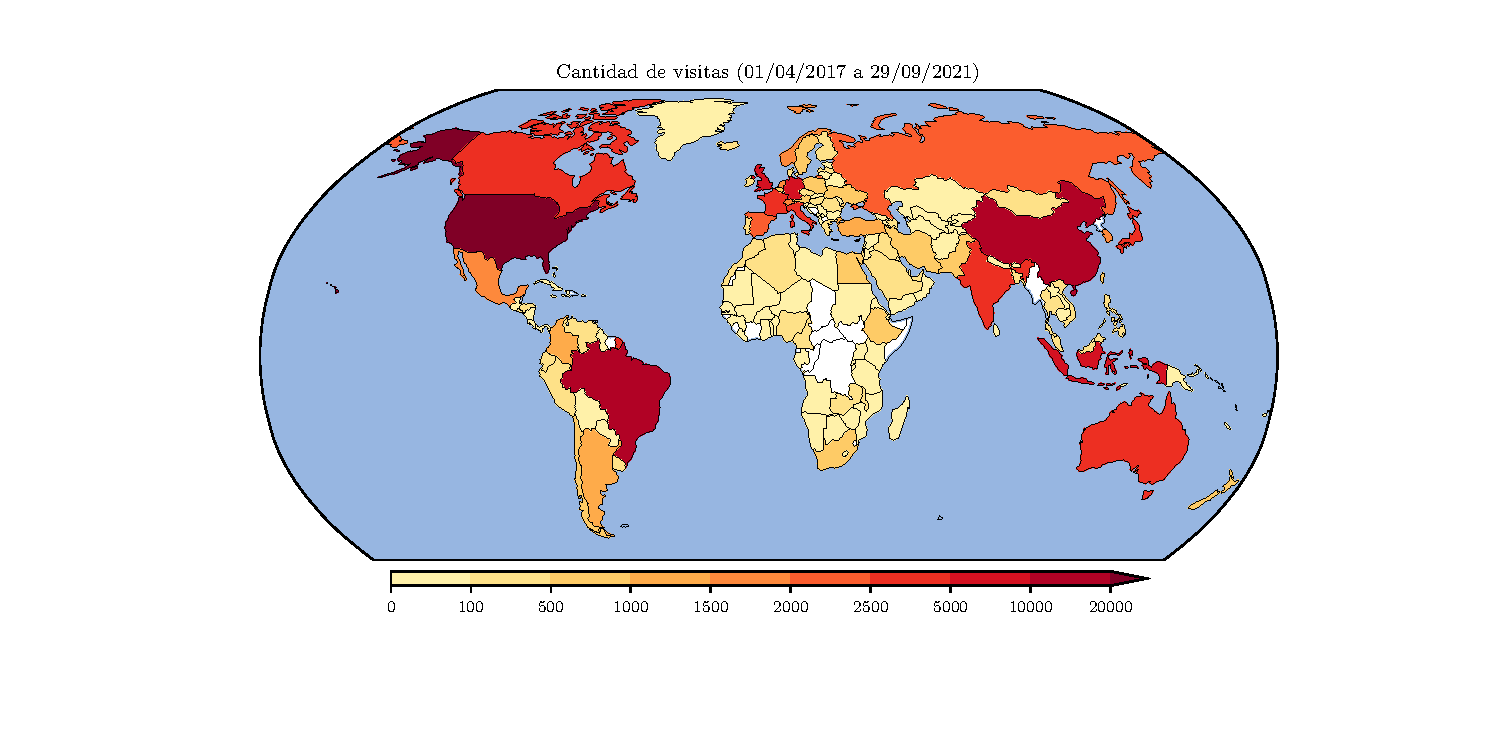
\includegraphics[width=\linewidth]{figs/fatiando/users_map.pdf}
    \caption{
        Cantidad de visitas a \href{https://fatiando.org}{fatiando.org} entre
        Abril de 2017 y Septiembre de 2021 por ubicación geográfica.
        Los países en grises con líneas paralelas blancas corresponden a sitios
        de los cuales no se han recibido visitas en el mismo período.
        La escala de colores posee pasos no proporcionales para mejorar la
        visualización del mapa.
    }
    \label{fig:fatiando-users-map}
\end{figure}

Estimar la cantidad de usuarios y usuarias que utilizan las herramientas que
ofrece el proyecto no es trivial.
Es posible conocer la cantidad de descargas de los paquetes desde PyPI
o \texttt{conda-forge}, sin embargo muchas de ellas son realizadas de manera
automática por servicios como los de integración continua, introduciendo una
sobreestimación de la cifra.
Quizás una métrica más representativa de esta variable es la cantidad de
visitas al sitio web \href{https://fatiando.org}{fatiando.org}, incluidas las
páginas de documentación.
Estos datos han sido recopilados mediante los servicios de Google Analytics de
manera anónima (no se recogen las direcciones de IP de quienes visitan el
sitio).
La figura~\ref{fig:fatiando-users-history} muestra la cantidad de visitas que
recibió el sitio desde Abril del 2017 a Septiembre de 2021 por ventana móvil de
28 días.
Mientras que la figura~\ref{fig:fatiando-users-map} expone la cantidad de
visitas en el mismo intervalo según su ubicación geográfica.

Estos datos ilustran que la cantidad de visitas experimenta una tendencia
ascendente, principalmente desde comienzos del 2019, con algunas variaciones
estacionales.
Además, podemos ver que países como Estados Unidos de América, Brasil y China
acaparan la mayor cantidad de consultas al sitio web del proyecto,
aunque el interés sobre el proyecto parece estar distribuido entre muchos
países del globo.


% \section{Planes a futuro}

% Stable release of every package

% Mayor interoperabilidad con el resto de paquetes geofísicos (SimPEG, pyGIMLi, etc)

% Implementar esféras en boule (luna, mercurio).
% Implementar elipsoides traixiales en boule.
% Unificar las clases de elipsoides para todo tipo.
